%! suppress = TooLargeSection
%! Author = cuj1559
%! Date = 26. 8. 29.

\documentclass[11pt,a4paper]{article}
\usepackage{hyperref}
\usepackage{tikz}
\usetikzlibrary{positioning}

\title{Staployfile Language Specification}
\author{Choiman1559}
\date{}

\begin{document}

    \maketitle

    \begin{center}
        Update Date: Aug 31, 2026 \\
        Version Based on Writing: 1.0.0 (93a8302)
    \end{center}

    \tableofcontents
    \newpage


    \section{Introduction}\label{sec:introduction}

    \subsection{Purpose}\label{subsec:purpose}

    Staployfile is a declarative configuration language used to describe
    application builds, package management, and deployment operations in the Staploy system.
    This specification defines the syntax and semantics of the Staployfile language.
    It describes the structure of a Staployfile, the meaning of its
    blocks and attributes, the resolution of aliases and other expressions,
    and the order in which operations are executed.
    The purpose of this specification is to provide a precise reference for
    users writing Staployfiles and for implementations processing them.
    Examples in this document are intended to illustrate the language syntax
    and execution semantics rather than prescribe a particular deployment environment.

    \subsection{Scope}\label{subsec:scope}

    This specification covers the following aspects of the Staployfile
    language:

    \begin{itemize}
        \item File and block structure based on HCL syntax.
        \item Global configuration through the \texttt{configure} block.
        \item Worker and application aliases through the \texttt{alias} block.
        \item Worker selection and filtering expressions.
        \item Multi-architecture application builds through the \texttt{build} block.
        \item Application management operations through the \texttt{manage} block.
        \item Deployment operations through the \texttt{target} block.
        \item Shell hooks executed before and after deployment operations.
        \item Alias and application reference resolution.
        \item Operation ordering and execution semantics.
        \item Errors encountered during parsing, resolution, building, and execution.
    \end{itemize}

    This specification does not define the Staploy server protocol, worker
    implementation, package archive format, or the internal implementation
    details of the Staploy CLI, except where those details are observable
    through the Staployfile language.

    \subsection{Terminology}\label{subsec:terminology}

    The following terms are used throughout this specification.

    \begin{description}
        \item[Staployfile]
        A configuration file written in the Staployfile language.
        It describes builds, package management operations, and deployment targets.

        \item[Worker]
        A Staploy worker process registered with a Staploy server.
        Workers are the execution targets for deployment operations.

        \item[Worker ID]
        The unique identifier assigned to a worker.

        \item[Worker Alias]
        A named expression representing one or more workers.
        A worker alias may contain explicit worker references, worker groups, and filtering
        conditions.

        \item[Application]
        A deployable package managed by Staploy.
        An application is identified by its name and, where applicable, its version.

        \item[App Alias]
        A named reference to an application name and optionally a version.
        App aliases may additionally be associated with the output of a build.

        \item[Build]
        An operation that produces a Staploy application package from one or
        more architecture-specific build outputs.

        \item[Manage Operation]
        An operation that manages an application package or its registration
        with the Staploy server, such as creating, uploading, deleting, or
        pulling a package.

        \item[Target]
        A named deployment definition specifying a set of workers and one or
        more operations to perform on those workers.

        \item[Target Operation]
        An operation performed against the workers selected by a target.
        Target operations include \texttt{unset}, \texttt{remove},
        \texttt{deploy}, \texttt{push\_only}, \texttt{set\_active}, and
        \texttt{disconnect}.

        \item[Shell Hook]
        A shell command executed as part of a target operation.
        Shell hooks may be executed before or after the main operation.

        \item[Alias Resolution]
        The process of converting an alias expression such as
        \texttt{alias:name} into the concrete worker or application reference
        represented by that alias.

        \item[Worker Expression]
        A string expression used to identify or select workers, including
        worker IDs, worker names, \texttt{group:} expressions, and
        \texttt{alias:} expressions.
    \end{description}


    \section{Language Overview}\label{sec:language-overview}

    \subsection{Staployfile}\label{subsec:staployfile}

    A Staployfile is a declarative configuration file that describes a
    sequence of application build, package management, and deployment operations.
    It consists of a set of top-level blocks.
    The principal blocks are \texttt{configure}, \texttt{alias}, \texttt{build}, \texttt{manage}, and \texttt{target}.
    Each block defines a distinct part of the desired build or deployment workflow.
    This does not directly describe the internal requests sent
    between the Staploy CLI, server, and workers.
    Instead, it describes the desired operations at a higher level.
    The Staploy CLI parses the file, resolves references and aliases, and translates the resulting
    declarations into executable operations.

    For example, a target may refer to a group of workers using a worker
    expression and may refer to an application using an application alias:

    \begin{center}
        %! suppress = MissingLabel
        \begin{verbatim}
            target "deploy_app" {
               workers = ["alias:production"]
               deploy "alias:my-app" {
                  post_deploy = "app --version"
               }
            }
        \end{verbatim}
    \end{center}

    The concrete workers, application name, and application version are
    resolved by the CLI before the corresponding operation is executed.

    \subsection{HCL Foundation}\label{subsec:hcl-foundation}

    Staployfile uses HCL (HashiCorp Configuration Language) as its syntactic foundation.
    Consequently, Staployfile inherits the basic HCL
    concepts of blocks, labels, attributes, expressions, and collections.
    The use of HCL provides a human-readable representation while allowing
    the Staployfile language to remain structured and extensible.
    Staployfile defines its own semantics on top of HCL. HCL syntax alone
    does not determine the meaning of a Staployfile.

    For example,
    \texttt{alias:production} and \texttt{group:all} are Staploy-specific
    worker expressions interpreted by the Staploy CLI. \\
    Accordingly, this specification distinguishes between the syntactic
    rules provided by HCL and the semantic rules defined by Staployfile.
    Unless otherwise specified, constructs described in this document are
    interpreted according to the Staployfile semantics.

    \subsection{Execution Model}\label{subsec:execution-model}

    The processing of a Staployfile consists of several conceptual stages.
    The CLI first parses the file into its corresponding configuration objects.
    It then initializes the execution context and resolves references required by subsequent operations.

    The general processing order is:

    \begin{enumerate}
        \item Parse the Staployfile.
        \item Apply the global configuration.
        \item Synchronize worker information with the Staploy server.
        \item Process worker and application aliases.
        \item Resolve build definitions and produce application packages.
        \item Execute application management operations.
        \item Resolve target worker and application references.
        \item Execute target operations.
    \end{enumerate}

    Alias resolution is performed before the operation that consumes the corresponding alias.
    Resolved information may be retained internally so that subsequent operations can reuse it without repeating the same resolution or server query.
    For each target, target operations are executed according to the defined operation precedence rather than the order in which the
    operations appear in the source file.

    The precedence is:

    \begin{center}
        \texttt{unset}
        $\rightarrow$
        \texttt{remove}
        $\rightarrow$
        \texttt{deploy}
        $\rightarrow$
        \texttt{push\_only}
        $\rightarrow$
        \texttt{set\_active}
        $\rightarrow$
        \texttt{disconnect}
    \end{center}

    Shell hooks associated with an operation are executed immediately before
    or after the corresponding operation, according to whether they are
    specified as \texttt{pre\_deploy} or \texttt{post\_deploy}.


    \section{File Syntax}\label{sec:file-syntax}

    \subsection{HCL Syntax}\label{subsec:hcl-syntax}

    Staployfile follows the syntax defined by HCL. A Staployfile is
    therefore composed of HCL blocks, labels, attributes, expressions, and values.
    This specification defines the semantic meaning of the HCL constructs used by Staployfile.
    Unless otherwise stated, lexical and syntactic rules are those of HCL.\\
    A minimal Staployfile may contain a single top-level block:

    \begin{center}
        %! suppress = MissingLabel
        \begin{verbatim}
            configure {
               address = "127.0.0.1"
               port    = 18090
            }
        \end{verbatim}
    \end{center}

    Multiple top-level blocks may be combined to describe a complete build
    and deployment workflow.

    \subsection{Blocks}\label{subsec:blocks}

    A block is a named structural element containing a set of nested
    attributes and, where applicable, child blocks.
    Staployfile defines the following top-level block types:

    \begin{itemize}
        \item \texttt{configure} --- defines global CLI and server configuration.
        \item \texttt{alias} --- defines worker and application aliases.
        \item \texttt{build} --- defines application package build operations.
        \item \texttt{manage} --- defines application management operations.
        \item \texttt{target} --- defines worker-targeted operations.
    \end{itemize}

    Some blocks may contain additional nested blocks.
    For example, a \texttt{target} may contain deployment operations:

    \begin{center}
        %! suppress = MissingLabel
        \begin{verbatim}
            target "production" {
               workers = ["group:all"]
               deploy "my-app" {
                  post_deploy = "my-app --version"
               }
            }
        \end{verbatim}
    \end{center}

    The set of valid child blocks and attributes is determined by the
    containing block and is specified in the corresponding sections of this document.

    \subsection{Labels}\label{subsec:labels}

    A label identifies a particular instance of a block.
    Labels are written immediately after the block type and are enclosed in quotation marks.
    For example:

    \begin{center}
        %! suppress = MissingLabel
        \begin{verbatim}
            build "my-app" {
               ...
            }

            target "production" {
               ...
            }
        \end{verbatim}
    \end{center}

    The interpretation of a label depends on the block in which it occurs.
    For example, the label of a \texttt{target} identifies the target, while
    the label of an \texttt{alias} child block identifies the alias name.
    Some blocks may accept multiple labels when required by the HCL schema.
    The number and meaning of labels supported by each block are defined in
    the relevant section of this specification.

    \subsection{Attributes}\label{subsec:attributes}

    An attribute assigns a value to a named property using the following form:

    \begin{center}
        %! suppress = MissingLabel
        \begin{verbatim}
            name = value
        \end{verbatim}
    \end{center}

    For example:

    \begin{center}
        %! suppress = MissingLabel
        \begin{verbatim}
            address      = "127.0.0.1"
            port         = 18090
            enforce_uuid = false
            workers      = ["worker-1", "worker-2"]
        \end{verbatim}
    \end{center}

    The type and interpretation of an attribute are determined by the block in which it appears.
    Attributes may contain primitive values such as strings, numbers, and
    booleans, as well as collections such as lists.
    Some attributes may also accept expressions evaluated by the Staploy CLI.\\
    An attribute may be optional, in which case its absence causes the
    implementation to use the default behavior defined for that attribute.

    \subsection{Expression}\label{subsec:expressions}

    Expressions are values whose meaning is interpreted by Staployfile or evaluated during execution.
    Staployfile defines several expression forms in addition to ordinary HCL values.
    A notable example is the worker expression:

    \begin{center}
        %! suppress = MissingLabel
        \begin{verbatim}
            workers = [
            "worker-1",
            "group:all",
            "alias:production"
            ]
        \end{verbatim}
    \end{center}

    The \texttt{group:} and \texttt{alias:} prefixes identify Staploy-specific expressions.
    These expressions are resolved according to the rules defined in the Worker Expressions and Resolution Rules sections.
    Application references may similarly use the \texttt{alias:} prefix:

    \begin{center}
        %! suppress = MissingLabel
        \begin{verbatim}
            deploy "alias:my-app" {
               ...
            }
        \end{verbatim}
    \end{center}

    Shell expressions may also be used by attributes that explicitly support shell evaluation.
    Such expressions are evaluated by the CLI at the stage defined by the corresponding operation.
    An expression is not necessarily evaluated when the file is parsed.
    Evaluation and resolution occur at the stage required by the semantics
    of the containing block or operation.


    \section{Global Blocks}\label{sec:global-blocks}

    A Staployfile is organized into a set of top-level blocks.
    Each block represents a distinct stage or component of the Staploy workflow.
    The following top-level blocks are defined:

    \begin{itemize}
        \item \texttt{configure}
        \item \texttt{alias}
        \item \texttt{build}
        \item \texttt{manage}
        \item \texttt{target}
    \end{itemize}

    Each block has a specific purpose and may contain a defined set of attributes and nested blocks.
    Blocks that are not recognized by the Staployfile implementation are rejected during parsing.

    \subsection{\texttt{configure}}\label{subsec:texttt{configure}}

    The \texttt{configure} block defines global configuration values used when processing the Staployfile.
    It may specify connection information for the Staploy server and global CLI behavior.
    Configuration defined in this block applies to operations within the current Staployfile unless overridden by an operation-specific mechanism.

    A typical configuration is:

    \begin{center}
        %! suppress = MissingLabel
        \begin{verbatim}
            configure {
               address      = "192.168.50.194"
               port         = 18090
               enforce_uuid = false
            }
        \end{verbatim}
    \end{center}

    The \texttt{configure} block is optional.
    When omitted, the CLI uses its default configuration and command-line configuration where applicable.

    \subsection{\texttt{alias}}\label{subsec:texttt{alias}}

    The \texttt{alias} block defines named references that can be reused
    throughout a Staployfile.

    Two alias types are currently supported:

    \begin{itemize}
        \item Worker aliases, which represent a set of workers.
        \item Application aliases, which represent an application name and,
        optionally, a version.
    \end{itemize}

    For example:

    \begin{center}
        %! suppress = MissingLabel
        \begin{verbatim}
            alias {
               worker "my-worker" {
                  workers = ["group:all"]
               }

               app "my-app" {
                  name    = "my-app"
                  version = "1.2.3"
               }
            }
        \end{verbatim}

    \end{center}

    Aliases are resolved when they are referenced by an operation.
    The detailed syntax and resolution rules for aliases are defined in Section~5.

    \subsection{\texttt{build}}\label{subsec:texttt{build}}

    The \texttt{build} block defines an application package build.
    A build describes the application name, output location, executable
    files, environment variables, architecture-specific build commands,
    and other metadata required to construct a Staploy package.

    For example:

    \begin{center}
        %! suppress = MissingLabel
        \begin{verbatim}
            build "my-app" {
               version = "1.2.3"
               output_dir = "zig-out"
               executable = ["my-app"]

               x86_64 {
                  pre_build = "./build-x86_64.sh"
                  path      = "zig-out/x86_64/bin"
               }
            }
        \end{verbatim}
    \end{center}

    A build may reference an application alias instead of specifying the
    application directly.

    \begin{center}
        %! suppress = MissingLabel
        \begin{verbatim}
            build "alias:my-app" {
               ...
            }
        \end{verbatim}
    \end{center}

    Build processing produces a package that may subsequently be consumed by a \texttt{manage} or \texttt{target} block.
    The complete build syntax is defined in Section~8.

    \subsection{\texttt{manage}}\label{subsec:texttt{manage}}

    The \texttt{manage} block defines operations that manage application
    packages independently of deployment to workers.
    Supported management operations include:

    \begin{itemize}
        \item \texttt{create}
        \item \texttt{upload}
        \item \texttt{delete}
        \item \texttt{pull}
    \end{itemize}

    For example:

    \begin{center}
        %! suppress = MissingLabel
        \begin{verbatim}
            manage "my-app" {
               upload {
                  package_file = "my-app.tar"
               }
            }
        \end{verbatim}
    \end{center}

    The application name may be specified directly or through an application alias.
    Management operations are executed after build processing and before target processing.
    Detailed management operation syntax is defined in Section~9.

    \subsection{\texttt{target}}\label{subsec:texttt{target}}

    The \texttt{target} block defines operations to be performed against a selected set of workers.
    A target has a label identifying the target and a \texttt{workers}
    attribute identifying the workers against which its operations are executed.

    For example:

    \begin{center}
        %! suppress = MissingLabel
        \begin{verbatim}
            target "production" {
               workers = ["alias:production"]
               deploy "my-app" {
                  post_deploy = "my-app --version"
               }
            }
        \end{verbatim}
    \end{center}

    A target may contain one or more target operations.
    The operations are processed according to the target operation precedence defined by this
    specification rather than by their textual order within the block.
    The currently supported target operations are:

    \begin{itemize}
        \item \texttt{unset}
        \item \texttt{remove}
        \item \texttt{deploy}
        \item \texttt{push\_only}
        \item \texttt{set\_active}
        \item \texttt{disconnect}
    \end{itemize}

    Each target operation MAY occur at most once within a target block.
    A target MUST NOT contain multiple blocks of the same operation type.
    For example, a target containing two \texttt{deploy} blocks is invalid.
    Different operation types MAY be specified together within the same target.
    This restriction applies independently to \texttt{unset}, \texttt{remove}, \texttt{deploy}, \texttt{push\_only}, \texttt{set\_active}, and \texttt{disconnect}.

    Target operations may also define shell hooks that are executed before or after the corresponding operation.
    Detailed target operation syntax and execution semantics are defined in Section~10.


    \section{Alias}\label{sec:alias}

    An alias provides a named reference to a set of resources or a specific application definition.
    Aliases allow other blocks to refer to resources without repeating their complete configuration.
    Aliases are declared in the global \texttt{alias} block and are resolved when a block references them using the \texttt{alias:} prefix.

    \subsection{Alias Model}\label{subsec:alias-model}

    The \texttt{alias} block defines named resources that can be referenced by other blocks in a Staployfile.
    An alias has a type and a name.
    The type determines the kind of resource represented by the alias.

    \begin{center}
        %! suppress = MissingLabel
        \begin{verbatim}
            alias {
               worker "my-workers" {
                  ...
               }

               app "my-app" {
                  ...
               }
            }
        \end{verbatim}
    \end{center}

    The following alias types are currently supported:

    \begin{itemize}
        \item \texttt{worker}: Defines a reusable worker selection.
        \item \texttt{app}: Defines a reusable application reference.
    \end{itemize}

    An alias is referenced by prefixing its name with \texttt{alias:}.

    \begin{center}
        %! suppress = MissingLabel
        \begin{verbatim}
            build "alias:my-app" {
               ...
            }

            manage "alias:my-app" {
               ...
            }

            target "deploy" {
               workers = ["alias:my-workers"]
               ...
            }
        \end{verbatim}
    \end{center}

    The \texttt{alias:} prefix explicitly indicates that the value is an alias reference rather than a literal resource name.

    \subsection{Worker Alias}\label{subsec:worker-alias}

    A worker alias represents a set of workers selected from the workers currently known to the Staploy server.
    A worker alias is declared using the \texttt{worker} block.

    \begin{center}
        %! suppress = MissingLabel
        \begin{verbatim}
            alias {
               worker "zmx-deploy" {
                  workers = ["group:all"]

                  where {
                     arch = ["x86_64", "arm", "aarch64", "mipsel"]
                  }
               }
        \end{verbatim}
    \end{center}

    The \texttt{workers} attribute specifies the initial worker selection.
    Worker groups may be used to select workers by group.
    The optional \texttt{where} block further filters the selected workers according to their worker information.
    For example, the following alias selects workers belonging to the \texttt{all} group whose architecture is supported by the application:

    \begin{center}
        %! suppress = MissingLabel
        \begin{verbatim}
            worker "zmx-deploy" {
               workers = ["group:all"]

               where {
                  arch = ["x86_64", "arm", "aarch64", "mipsel"]
               }
            }
        \end{verbatim}
    \end{center}

    Worker aliases are resolved against the workers known to the server when the Staployfile is processed.
    Therefore, the result of a worker alias may differ as workers join, leave, or change their reported properties.
    A worker alias can be used wherever a worker selection is accepted.

    \begin{center}
        %! suppress = MissingLabel
        \begin{verbatim}
            target "upload_zmx" {
               workers = ["alias:zmx-deploy"]
            }
        \end{verbatim}
    \end{center}

    \subsection{App Alias}\label{subsec:app-alias}

    An application alias provides a reusable reference to an application and its version information.
    An app alias is declared using the \texttt{app} block.

    \begin{center}
        %! suppress = MissingLabel
        \begin{verbatim}
            alias {
               app "zmx-build" {
                  name = "zmx"
                  version = "shell:git describe --tags --abbrev=0"
               }
            }
        \end{verbatim}
    \end{center}

    The \texttt{name} attribute specifies the application name registered in the Staploy server.
    The \texttt{version} attribute specifies the version associated with the application.
    The value may be resolved dynamically using a supported value expression such as a shell command.
    An app alias can be referenced by build, management, and deployment blocks.

    \begin{center}
        %! suppress = MissingLabel
        \begin{verbatim}
            build "alias:zmx-build" {
               ...
            }

            manage "alias:zmx-build" {
               ...
            }

            target "upload_zmx" {
               deploy "alias:zmx-build" {
                  ...
               }
            }
        \end{verbatim}
    \end{center}

    Using an app alias allows the same application definition to be shared by multiple stages of a Staployfile without duplicating the application name or version definition.
    This is particularly useful when a build artifact is subsequently registered and deployed as part of the same workflow.

    \subsection{Alias Resolution}\label{subsec:alias-resolution}

    Alias references are resolved when the Staployfile is processed.
    An alias reference has the form of \texttt{alias:[ALIAS\_NAME]}.
    The alias name is resolved within the aliases declared in the current Staployfile.
    The resolved alias must have a type compatible with the context in which it is referenced.
    For example, a worker alias may be used as a worker selection:

    \begin{center}
        %! suppress = MissingLabel
        \begin{verbatim}
            target "upload_zmx" {
               workers = ["alias:zmx-deploy"]
            }
        \end{verbatim}
    \end{center}

    while an app alias may be used as an application reference:

    \begin{center}
        %! suppress = MissingLabel
        \begin{verbatim}
            build "alias:zmx-build" {
               ...
            }
        \end{verbatim}
    \end{center}

    An alias reference does not itself create a new worker or application.
    It only provides an indirect reference to the corresponding alias definition.
    If an alias cannot be resolved, or if an alias of an incompatible type is used,
    processing of the Staployfile fails with an appropriate configuration error.
    Alias resolution also provides a separation between resource selection and resource execution.
    For example, a worker alias determines which workers participate in a target, while the target itself determines what operation is performed on those workers.
    This allows a single alias to be reused by multiple blocks while keeping resource selection independent of the execution workflow.


    \section{Worker Expressions}\label{sec:worker-expressions}

    Worker expression specify the workers to which an operation is applied.
    A worker expression may identify a worker directly, select workers through a group, or refer to a previously defined worker alias.
    Worker expressions are used by blocks that operate on one or more workers, including target operations.

    \subsection{Worker ID}\label{subsec:worker-id}

    A worker ID identifies a worker by its unique identifier assigned by Staploy.
    A worker ID may be specified directly in a worker expression.

    \begin{center}
        %! suppress = MissingLabel
        \begin{verbatim}
            target "deploy" {
               workers = ["worker-8f3c2a"]
            }
        \end{verbatim}
    \end{center}

    Worker IDs are expected to uniquely identify a worker.
    The worker ID is resolved against the workers known to the Staploy server.
    If a specified worker ID does not correspond to a known worker, the worker expression cannot be resolved.

    \subsection{Worker Name}\label{subsec:worker-name}

    A worker name identifies a worker using its configured or reported name.
    A worker name may be used where a worker expression accepts a direct worker reference.

    \begin{center}
        %! suppress = MissingLabel
        \begin{verbatim}
            target "deploy" {
               workers = ["zmx-worker-01"]
            }
        \end{verbatim}
    \end{center}

    Unlike a worker ID, a worker name is not necessarily a globally unique identifier.
    If multiple workers match the specified name, the implementation MUST apply the worker resolution rules defined by the execution context.
    Worker names are therefore intended primarily for human-readable worker references.
    Worker IDs SHOULD be preferred when an unambiguous reference to a specific worker is required.

    \subsection{\texttt{group:} Expression}\label{subsec:texttts-expression}

    The \texttt{group:} expression selects workers belonging to a worker group.
    The general form is: \texttt{group:[GROUP\_NAME]}
    For example:

    \begin{center}
        %! suppress = MissingLabel
        \begin{verbatim}
            target "deploy" {
               workers = ["group:production"]
            }
        \end{verbatim}
    \end{center}

    A group expression represents a set of workers rather than a single worker.
    The set is determined from the workers known to the Staploy server and their associated group information.
    The special group name \texttt{all}, when supported by the implementation, represents all workers available to the current operation.

    \begin{center}
        %! suppress = MissingLabel
        \begin{verbatim}
            target "deploy" {
               workers = ["group:all"]
            }
        \end{verbatim}
    \end{center}

    Group expressions may be combined with other worker expressions in the same worker selection.

    \begin{center}
        %! suppress = MissingLabel
        \begin{verbatim}
            target "deploy" {
               workers = [
               "worker-8f3c2a",
               "group:production"
               ]
            }
        \end{verbatim}
    \end{center}

    The resulting worker set is resolved before the corresponding operation is executed.

    \subsection{\texttt{alias:} Expression}\label{subsec:texttt-expression}

    The \texttt{alias:} expression refers to a worker alias declared in the Staployfile.
    The general form is: \texttt{alias:[ALIAS\_NAME]}.

    For example:

    \begin{center}
        %! suppress = MissingLabel
        \begin{verbatim}
            alias {
               worker "production-workers" {
                  workers = ["group:production"]
               }
            }

            target "deploy" {
               workers = ["alias:production-workers"]
            }
        \end{verbatim}
    \end{center}

    A worker alias is resolved to the worker selection defined by the corresponding alias declaration.
    The \texttt{alias:} prefix distinguishes an alias reference from a direct worker ID, worker name, or group expression.
    An \texttt{alias:} expression MUST refer to a worker alias when used in a worker expression.
    Referencing an application alias or an undefined alias is a resolution error.

    \subsection{\texttt{where} Block}\label{subsec:where-block}

    The \texttt{where} block filters a set of workers according to their reported attributes.
    A \texttt{where} block is applied to a worker selection obtained from a worker expression.
    Each condition specifies a constraint on one worker attribute.

    \begin{center}
        %! suppress = MissingLabel
        \begin{verbatim}
            target "deploy" {
               workers = ["group:all"]

               where {
                  arch = ["x86_64"]
                  memory = "20G.."
                  cpu = "!..10"
                  name = "prefix:cuj1559-vm"
               }
            }
        \end{verbatim}
    \end{center}

    All conditions specified in the same \texttt{where} block are combined conjunctively.
    A worker therefore remains in the resulting worker set only when it satisfies every specified condition.

    \subsubsection{Worker Attributes}

    The following worker attributes may be used as \texttt{where} conditions:

    \begin{description}
        \item[\texttt{name}]
        The worker name.

        \item[\texttt{arch}]
        The CPU architecture reported by the worker.
        Multiple values may be specified.

        \item[\texttt{cpu}]
        The CPU information reported by the worker.

        \item[\texttt{memory}]
        The memory information reported by the worker.

        \item[\texttt{workdir}]
        The working directory reported by the worker.

        \item[\texttt{shell\_enable}]
        Whether shell execution is enabled for the worker.

        \item[\texttt{integrity\_skip}]
        Whether integrity checking is skipped for the worker.
    \end{description}

    Boolean attributes such as \texttt{shell\_enable} and \texttt{integrity\_skip} are specified as boolean values.

    \begin{center}
        %! suppress = MissingLabel
        \begin{verbatim}
            where {
               shell_enable = true
               integrity_skip = false
            }
        \end{verbatim}
    \end{center}

    String and numeric attributes support filter expressions.
    The expression determines how the supplied value is compared with the corresponding worker attribute.

    \subsubsection{Exact Matching}

    The \texttt{exact:} prefix explicitly requests an exact string match.

    \begin{center}
        %! suppress = MissingLabel
        \begin{verbatim}
            where {
               name = "exact:cuj1559-vm-01"
            }
        \end{verbatim}
    \end{center}

    The condition is satisfied only when the complete attribute value is equal to the specified value.
    The \texttt{exact:} prefix is useful when a more general string matching rule could otherwise be applicable.
    If no filter prefix is specified for a string attribute, the condition
    is interpreted as an exact match.

    \subsubsection{Prefix Matching}

    The \texttt{prefix:} prefix matches strings beginning with the specified value.

    \begin{center}
        %! suppress = MissingLabel
        \begin{verbatim}
            where {
               name = "prefix:cuj1559-vm"
            }
        \end{verbatim}
    \end{center}

    The condition above matches worker names such as \texttt{cuj1559-vm-01} and \texttt{cuj1559-vm-02}, provided that the complete worker name begins with \texttt{cuj1559-vm}.

    \subsubsection{Suffix Matching}

    The \texttt{suffix:} prefix matches strings ending with the specified value.

    \begin{center}
        %! suppress = MissingLabel
        \begin{verbatim}
            where {
               name = "suffix:-prod"
            }
        \end{verbatim}
    \end{center}

    The condition matches worker names whose complete value ends with \texttt{-prod}.

    \subsubsection{Regular Expression Matching}

    The \texttt{regex:} prefix interprets the remainder of the expression as a regular expression.

    \begin{center}
        %! suppress = MissingLabel
        \begin{verbatim}
            where {
               name = "regex:^cuj[0-9]+-vm-[0-9]+$"
            }
        \end{verbatim}
    \end{center}

    A worker satisfies the condition when the corresponding attribute matches the specified regular expression.
    The regular expression syntax and behavior are determined by the regular expression implementation used by Staploy.

    \subsubsection{Numeric Range Matching}

    Numeric attributes support range expressions using the \texttt{\string.\string.} operator.
    A range may specify a lower bound, an upper bound, or both.

    \begin{center}
        %! suppress = MissingLabel
        \begin{verbatim}
            where {
               memory = "20G.."
            }
        \end{verbatim}
    \end{center}

    The expression above specifies a lower-bounded range and matches values greater than or equal to \texttt{20G}.
    An upper-bounded range may be specified by placing \texttt{\string.\string.} before the value.

    \begin{center}
        %! suppress = MissingLabel
        \begin{verbatim}
            where {
               memory = "..64G"
            }
        \end{verbatim}
    \end{center}

    A bounded range may specify both endpoints.

    \begin{center}
        %! suppress = MissingLabel
        \begin{verbatim}
            where {
               memory = "4G..64G"
            }
        \end{verbatim}
    \end{center}

    The range operator is primarily intended for numeric worker attributes such as memory and CPU-related values.

    \subsubsection{Negation}

    The \texttt{!} prefix negates a filter expression.

    \begin{center}
        %! suppress = MissingLabel
        \begin{verbatim}
            where {
               name = "!prefix:test-"
            }
        \end{verbatim}
    \end{center}

    The condition above matches worker names that do not satisfy the \texttt{prefix:test} expression.
    Negation may be combined with other filter expressions.

    For example:

    \begin{center}
        %! suppress = MissingLabel
        \begin{verbatim}
            where {
               cpu = "!..10"
            }
        \end{verbatim}
    \end{center}

    This applies the negated form of the corresponding range expression.

    \subsubsection{Filter Selection}

    The filter operators are summarized below.

    \begin{center}
        \begin{tabular}{ll}
            \textbf{Expression}   & \textbf{Meaning}                \\
            \hline
            \texttt{exact:VALUE}  & Exact string match              \\
            \texttt{prefix:VALUE} & Prefix string match             \\
            \texttt{suffix:VALUE} & Suffix string match             \\
            \texttt{regex:EXPR}   & Regular expression match        \\
            \texttt{VALUE..}      & Lower-bounded numeric range     \\
            \texttt{..VALUE}      & Upper-bounded numeric range     \\
            \texttt{VALUE..VALUE} & Bounded numeric range           \\
            \texttt{!EXPR}        & Negation of a filter expression \\
        \end{tabular}
    \end{center}

    These expressions may be used wherever the corresponding worker attribute supports the relevant comparison operation.
    An implementation MUST reject a filter expression that is not applicable to the type of the selected worker attribute.
    For example, a numeric range expression MUST NOT be interpreted as a string prefix or suffix expression merely because the attribute is represented as a string in the Staployfile.

    \subsubsection{Combined Conditions}

    Multiple conditions may be combined to construct a more specific worker selection.

    \begin{center}
        %! suppress = MissingLabel
        \begin{verbatim}
            target "filter_test" {
               workers = ["group:all"]

               where {
                  arch = ["x86_64"]
                  memory = "20G.."
                  cpu = "!..10"
                  name = "prefix:cuj1559-vm"
               }

               set_active "staploy-worker" {
                  version = "1.0.0"
               }
            }
        \end{verbatim}
    \end{center}

    The example selects workers satisfying all the following conditions:

    \begin{itemize}
        \item the worker architecture is \texttt{x86\_64};
        \item the worker has at least \texttt{20G} of memory;
        \item the worker's CPU value does not satisfy the specified upper-bounded range;
        \item the worker name begins with \texttt{cuj1559-vm}.
    \end{itemize}

    The \texttt{where} block does not itself select the initial worker population.
    Instead, it filters the workers produced by the preceding worker expression.
    If no worker satisfies the combined conditions, the resulting worker set is empty.
    The handling of an empty worker set is determined by the operation using the worker selection.

    If worker resolution or filtering produces an empty worker set,
    the target is skipped and reported as having no matching workers.
    The target MUST NOT be reported as successfully executed.


    \section{Application References}\label{sec:application-references}

    Application reference identifies an application and, when required, a specific version to be used by an operation.
    An application reference may identify an application directly, refer to an application alias, or obtain a version from a shell command.

    \subsection{Application Name}\label{subsec:application-name}

    An application name identifies an application registered on the Staploy server.
    It is specified as the application identifier in an operation that accepts an application reference.

    \begin{center}
        %! suppress = MissingLabel
        \begin{verbatim}
            set_active "staploy-worker" {
               version = "1.0.0"
            }
        \end{verbatim}
    \end{center}

    The application name is resolved against the applications known to the Staploy server.
    If no application with the specified name exists, application resolution fails.

    \subsection{Application Version}\label{subsec:application-version}

    An application version identifies a specific version of an application.

    \begin{center}
        %! suppress = MissingLabel
        \begin{verbatim}
            set_active "staploy-worker" {
               version = "1.0.0"
            }
        \end{verbatim}
    \end{center}

    The version value is interpreted as an application version identifier.
    The specified version MUST be available for the referenced application when the operation requires an existing application artifact.
    Version selection is independent of worker selection.
    If an operation targets multiple workers with different architectures,
    the selected application version MUST provide an artifact compatible with each worker to which the operation is applied.

    \subsection{\texttt{alias:} Expression}\label{subsec:texttt-expression2}

    The \texttt{alias:} expression refers to an application alias declared in the Staployfile.
    For example:

    \begin{center}
        %! suppress = MissingLabel
        \begin{verbatim}
            alias {
               app "latest-worker" {
                  name = "staploy-worker"
                  version = "1.0.0"
               }
            }
        \end{verbatim}
    \end{center}

    An application alias is resolved to the application reference represented by the corresponding alias declaration.
    The \texttt{alias:} prefix explicitly identifies the reference as an alias.
    A worker alias MUST NOT be used where an application reference is required, and an undefined application alias results in a resolution error.

    \subsection{\texttt{shell:} Expression}\label{subsec:texttt-shell-expression}

    The \texttt{shell:} expression obtains an application reference value by executing a shell command.

    The general form is:

    \begin{center}
        %! suppress = MissingLabel
        \begin{verbatim}
            shell:
        \end{verbatim}
    \end{center}

    For example:

    \begin{center}
        %! suppress = MissingLabel
        \begin{verbatim}
            alias {
                app "staploy-worker" {
                    version = "shell:git describe --tags --abbrev=0"
                }
            }
        \end{verbatim}
    \end{center}

    The shell command is executed by the Staploy client and its resulting output is used as the value of the corresponding application reference.
    This permits application versions to be determined dynamically rather than being hard-coded in the Staployfile.
    For example, a project may derive the version from a Git tag or another external versioning mechanism.
    The command MUST complete successfully for the expression to resolve successfully.
    The resulting value is interpreted according to the context in which the \texttt{shell:} expression occurs.
    Shell expressions are evaluated during execution of the corresponding operation.
    Consequently, their result may differ between executions of the same Staployfile.
    The use of \texttt{shell:} expressions may depend on the shell execution environment of the Staploy client.
    Implementations SHOULD document the shell, environment variables, working directory, and output handling used when evaluating shell expressions.


    \section{Build}\label{sec:build}

    The \texttt{build} block defines the procedure for producing an application package.
    A build specifies the application name, output directory, executable files, build environment,
    optional version information, and one or more target configurations.
    A build may contain architecture-specific targets as well as files shared by all targets.
    Build commands may be specified globally or for an individual target.

    \subsection{Build Block}\label{subsec:build-block}

    A build block is identified by an application name and has the following general form:

    \begin{center}
        %! suppress = MissingLabel
        \begin{verbatim}
            build "my-app" {
               output_dir = "./build"
               executable = ["my-app"]

               x86_64 {
                  path = "./bin/amd64"
               }
            }
        \end{verbatim}
    \end{center}

    The label of the build block specifies the application name to which the resulting artifacts belong.
    A build block may contain the following attributes and target blocks:

    \begin{itemize}
        \item \texttt{output\_dir}
        \item \texttt{version}
        \item \texttt{executable}
        \item \texttt{envs}
        \item \texttt{lib\_version}
        \item \texttt{pre\_build}
        \item \texttt{post\_build}
        \item \texttt{share}
        \item architecture-specific target blocks
    \end{itemize}

    The \texttt{output\_dir} and \texttt{executable} attributes define the basic output of a build.
    Target blocks determine which files are associated with each target architecture.

    \subsection{Build Attributes}\label{subsec:build-attributes}

    \subsubsection{\texttt{output\_dir}}

    The \texttt{output\_dir} attribute specifies the directory used as the output of the build.

    \begin{center}
        %! suppress = MissingLabel
        \begin{verbatim}
            build "my-app" {
               output_dir = "./build"
               ...
            }
        \end{verbatim}
    \end{center}

    The output directory is used as the base location from which the resulting application files are collected.

    \subsubsection{\texttt{version}}

    The optional \texttt{version} attribute specifies the version associated with the resulting application.

    \begin{center}
        %! suppress = MissingLabel
        \begin{verbatim}
            build "my-app" {
               output_dir = "./build"
               version = "1.2.0"
               ...
            }
        \end{verbatim}
    \end{center}

    If omitted, the version may be determined by the surrounding build or application resolution semantics.

    \subsubsection{\texttt{executable}}

    The \texttt{executable} attribute specifies the names of executable files contained in the resulting application.

    The values are file names rather than filesystem paths.

    \begin{center}
        %! suppress = MissingLabel
        \begin{verbatim}
            build "my-app" {
               output_dir = "./build"

               executable = [
               "my-app",
               "helper"
               ]
               ...
            }
        \end{verbatim}
    \end{center}

    The specified names are registered as executable files in the resulting application package.
    They identify files in the build output and are not interpreted as source paths.

    \subsubsection{\texttt{envs}}

    The optional \texttt{envs} attribute specifies environment variables used while executing the build.

    \begin{center}
        %! suppress = MissingLabel
        \begin{verbatim}
            build "my-app" {
               output_dir = "./build"

               envs = [
               "CGO_ENABLED=0",
               "GOFLAGS=-trimpath"
               ]

               ...
            }
        \end{verbatim}
    \end{center}

    The supplied values are passed to the build environment according to the shell execution semantics of the implementation.

    \subsubsection{\texttt{lib\_version}}

    The optional \texttt{lib\_version} attribute specifies the library version associated with the build.

    \begin{center}
        %! suppress = MissingLabel
        \begin{verbatim}
            build "my-app" {
               output_dir = "./build"
               lib_version = "1.4.0"
               ...
            }
        \end{verbatim}
    \end{center}

    The interpretation of this value is dependent on the application and its build process.

    \subsection{Target Architectures}\label{subsec:target-architectures}

    Architecture-specific build targets are represented by nested blocks.
    Each target identifies the files and optional commands associated with one architecture.
    The following architecture-specific target blocks are supported:

    \begin{center}
        \begin{tabular}{ll}
            \textbf{Block}    & \textbf{Architecture}     \\
            \hline
            \texttt{i386}     & 32-bit x86                \\
            \texttt{x86\_64}  & 64-bit x86                \\
            \texttt{arm}      & 32-bit ARM                \\
            \texttt{aarch64}  & 64-bit ARM                \\
            \texttt{riscv32}  & 32-bit RISC-V             \\
            \texttt{riscv64}  & 64-bit RISC-V             \\
            \texttt{mipsel}   & Little-endian MIPS        \\
            \texttt{mips64el} & 64-bit little-endian MIPS \\
        \end{tabular}
    \end{center}

    A target block has the following form:

    \begin{center}
        %! suppress = MissingLabel
        \begin{verbatim}
            x86_64 {
               path = "./bin/amd64"
            }
        \end{verbatim}
    \end{center}

    The \texttt{path} attribute identifies the path containing the files associated with the target.
    Different target blocks may therefore refer to different build outputs.

    \begin{center}
        %! suppress = MissingLabel
        \begin{verbatim}
            build "my-app" {
               output_dir = "./build"

               x86_64 {
                  path = "./bin/amd64"
               }

               aarch64 {
                  path = "./bin/arm64"
               }
            }
        \end{verbatim}
    \end{center}

    The resulting application package for each architecture is constructed from the corresponding architecture-specific target together with the files specified by the \texttt{share} block.

    \subsubsection{\texttt{share} Target}

    The \texttt{share} block specifies files common to all target architectures.

    Unlike an architecture-specific target, \texttt{share} does not represent a CPU architecture.
    Its contents are included in the output of every architecture-specific target.

    \begin{center}
        %! suppress = MissingLabel
        \begin{verbatim}
            build "my-app" {
               output_dir = "./build"

               share {
                  path = "./resources"
               }

               x86_64 {
                  path = "./bin/amd64"
               }

               aarch64 {
                  path = "./bin/arm64"
               }
            }
        \end{verbatim}
    \end{center}

    In this example, the files contained in \texttt{./resources} are shared by both the \texttt{x86\_64} and \texttt{aarch64} outputs.
    A shared file is therefore not required to be duplicated in each architecture-specific target.

    \subsection{Pre-build Commands}\label{subsec:pre-build-commands}

    The \texttt{pre\_build} attribute specifies a command to be executed before the corresponding build stage.
    A build-level \texttt{pre\_build} command applies to the build as a whole.

    \begin{center}
        %! suppress = MissingLabel
        \begin{verbatim}
            build "my-app" {
               output_dir = "./build"
               pre_build = "go generate ./..."

               ...
            }
        \end{verbatim}
    \end{center}

    A target may additionally define its own \texttt{pre\_build} command.

    \begin{center}
        %! suppress = MissingLabel
        \begin{verbatim}
            build "my-app" {
               output_dir = "./build"

               x86_64 {
                  path = "./bin/amd64"
                  pre_build = "make build-amd64"
               }
            }
        \end{verbatim}
    \end{center}

    A target-level command applies only to the corresponding target, while a build-level command applies to the build as a whole.
    The order in which build-level and target-level commands are executed is defined by the execution semantics of the build processor.

    \subsection{Build Output}\label{subsec:build-output}

    The build output consists of the files collected from the selected target and the corresponding \texttt{share} target.
    For an architecture-specific target, the target's \texttt{path} identifies the target-specific files.

    \begin{center}
        %! suppress = MissingLabel
        \begin{verbatim}
            build "my-app" {
               output_dir = "./build"

               executable = [
               "my-app"
               ]

               share {
                  path = "./resources"
               }

               x86_64 {
                  path = "./bin/amd64"
               }
            }
        \end{verbatim}
    \end{center}

    The resulting output contains both the architecture-specific files from \texttt{./bin/amd64} and the shared files from \texttt{./resources}.

    The \texttt{executable} attribute does not specify the source location of these files.
    It specifies which resulting files are considered executable files.
    If the expected build output cannot be located or processed, the build operation fails.
    The resulting artifacts are subsequently available to operations such as upload and deployment through build artifact resolution.

    \subsection{Build Alias Resolution}\label{subsec:build-alias-resolution}

    A build may be referenced indirectly through an application alias.
    When an application reference resolves to an application associated with a build definition,
    the corresponding build definition may be used to produce the application artifact.
    Build alias resolution therefore connects an application reference with the build definition that produces its artifact.

    For example:

    \begin{center}
        %! suppress = MissingLabel
        \begin{verbatim}
            alias {
               app "my-app" {
                  ...
               }
            }

            build "my-app" {
               output_dir = "./build"

               executable = [
               "my-app"
               ]

               x86_64 {
                  path = "./bin/amd64"
               }
            }
        \end{verbatim}
    \end{center}

    The alias does not modify the build definition.
    It provides an alternative name through which the application or build can be referenced.
    If an alias cannot be resolved to a valid application or build definition, the corresponding operation fails during resolution.
    Build alias resolution precedes build artifact resolution.
    The former identifies the application and its associated build definition,
    while the latter identifies the concrete artifact corresponding to the target architecture.


    \section{Manage Operations}\label{sec:manage-operations}

    The \texttt{manage} block defines operations for managing applications and application packages in the local Staploy server.
    A manage block is associated with an application by its label:

    \begin{center}
        %! suppress = MissingLabel
        \begin{verbatim}
            manage "my-app" {
               ...
            }
        \end{verbatim}
    \end{center}

    A \texttt{manage} block may contain one or more of the following operations:

    \begin{itemize}
        \item \texttt{create} --- create an application in the local Staploy server.
        \item \texttt{upload} --- upload a local application package to the local Staploy server.
        \item \texttt{delete} --- delete application versions from the local Staploy server.
        \item \texttt{pull} --- import an application package from an external Staploy repository into the local Staploy server.
    \end{itemize}

    Each operation is independent and is executed only when explicitly specified.

    \subsection{Manage Block}\label{subsec:manage-block}

    The general form of a \texttt{manage} block is:

    \begin{center}
        %! suppress = MissingLabel
        \begin{verbatim}
            manage "my-app" {
               create {
                  ...
               }

               upload {
                  ...
               }

               delete {
                  ...
               }

               pull "my-app" {
                  ...
               }
            }
        \end{verbatim}
    \end{center}

    The label of the \texttt{manage} block identifies the application to which the management operations apply.
    The operations may be combined in a single block.
    They are processed according to the execution semantics defined in Section~\ref{sec:execution-semantics}.

    \subsection{\texttt{create}}\label{subsec:texttt}

    The \texttt{create} operation creates an application in the local Staploy server.
    It accepts an optional \texttt{description} attribute:

    \begin{center}
        %! suppress = MissingLabel
        \begin{verbatim}
            manage "my-app" {
               create {
                  description = "My application"
               }
            }
        \end{verbatim}
    \end{center}

    The \texttt{description} attribute specifies the description associated with the application.
    If omitted, the application is created without an explicitly specified description.
    The application is created in the local Staploy server to which the operation is submitted.

    \subsection{\texttt{upload}}\label{subsec:texttt:upload}

    The \texttt{upload} operation uploads an application package from the local filesystem to the local Staploy server.
    It accepts an optional \texttt{path} attribute specifying the package file:

    \begin{center}
        %! suppress = MissingLabel
        \begin{verbatim}
            manage "my-app" {
               upload {
                  path = "./build/my-app.tar"
               }
            }
        \end{verbatim}
    \end{center}

    The \texttt{path} attribute identifies the local package file to upload.
    If \texttt{path} is omitted, the package is resolved according to the applicable build artifact resolution rules.
    The package is transferred to the local Staploy server and registered as a version of the application identified by the enclosing \texttt{manage} block.
    The operation does not upload the package to an external repository.
    The destination is always the local Staploy server associated with the current execution.

    \subsection{\texttt{delete}}\label{subsec:texttt:delete}

    The \texttt{delete} operation deletes application versions from the local Staploy server.
    Specific versions may be specified using the \texttt{versions} attribute:

    \begin{center}
        %! suppress = MissingLabel
        \begin{verbatim}
            manage "my-app" {
               delete {
                  versions = [
                  "1.0.0",
                  "1.1.0"
                  ]
               }
            }
        \end{verbatim}
    \end{center}

    Each value identifies an application version to be deleted.

    If the \texttt{versions} attribute is omitted, all versions of the application are deleted.

    \begin{center}
        %! suppress = MissingLabel
        \begin{verbatim}
            manage "my-app" {
               delete {}
            }
        \end{verbatim}
    \end{center}

    An empty \texttt{delete} block therefore represents an explicit request to delete all versions of the application.
    The operation applies to the application identified by the label of the enclosing \texttt{manage} block.

    \subsection{\texttt{pull}}\label{subsec:texttt:pull}

    The \texttt{pull} operation imports an application package from an external Staploy repository into the local Staploy server.
    The application to import is identified by the label of the \texttt{pull} block:

    \begin{center}
        %! suppress = MissingLabel
        \begin{verbatim}
            manage "my-app" {
               pull "my-app" {
                  version = "1.2.0"
                  repository = "https://repository.example.com"
               }
            }
        \end{verbatim}
    \end{center}

    The \texttt{name} label identifies the application to retrieve from the external repository.
    The optional \texttt{version} attribute specifies the application version to import.
    If omitted, the version is resolved according to the application resolution rules.
    The \texttt{repository} attribute specifies the URL of the external Staploy repository.
    The operation retrieves the requested application package from the external repository and registers it in the local Staploy server.

    For example:

    \begin{center}
        %! suppress = MissingLabel
        \begin{verbatim}
            manage "my-app" {
               pull "my-app" {
                  repository = "https://repository.example.com"
               }
            }
        \end{verbatim}
    \end{center}

    In contrast to \texttt{upload}, which transfers a package from the local filesystem to the local server, \texttt{pull} transfers an application package from an external Staploy repository to the local server.
    The \texttt{pull} operation therefore does not merely download a package to the local filesystem.
    The retrieved application and package are registered in the local Staploy server and can subsequently be managed or deployed using the local repository.
    The specified \texttt{repository} MUST identify an accessible Staploy repository endpoint.
    If the requested application or version cannot be resolved in the external repository, or if the package cannot be retrieved or registered in the local server, the \texttt{pull} operation fails.


    \section{Target Operations}\label{sec:target-operations}

    The \texttt{target} block defines operations to be performed on one or more workers.
    A target consists of a worker selection and one or more operations.
    The selected workers are determined by the \texttt{workers} attribute and, optionally, a \texttt{where} block.

    \subsection{Target Block}\label{subsec:target-block}

    A \texttt{target} block is identified by a label and contains the workers on which its operations are performed.

    \begin{center}
        %! suppress = MissingLabel
        \begin{verbatim}
            target "production" {
               workers = ["group:production"]

               deploy "my-app" {
                  version = "1.2.0"
               }
            }
        \end{verbatim}
    \end{center}

    The \texttt{workers} attribute specifies the initial set of workers targeted by the block.
    A target may contain multiple operations.
    Each operation is applied to the workers selected by the target.

    \subsection{Worker Selection}\label{subsec:worker-selection}

    Workers are selected using the \texttt{workers} attribute:

    \begin{center}
        %! suppress = MissingLabel
        \begin{verbatim}
            target "production" {
               workers = [
               "worker-01",
               "worker-02",
               "worker-03"
               ]

               ...
            }
        \end{verbatim}
    \end{center}

    Worker expressions may refer to worker IDs, worker names, groups, or aliases.
    Multiple expressions may be specified simultaneously.
    A \texttt{where} block may be used to further restrict the selected workers:

    \begin{center}
        %! suppress = MissingLabel
        \begin{verbatim}
            target "production" {
               workers = ["group:all"]

               where {
                  arch   = ["x86_64"]
                  memory = "20G.."
                  cpu    = "!..10"
                  name   = "prefix:production-"
               }

               ...
            }
        \end{verbatim}
    \end{center}

    The \texttt{where} conditions are applied to the workers selected by \texttt{workers}.
    A worker must satisfy the specified conditions to remain in the target set.
    If multiple conditions are specified, all conditions must be satisfied.
    The syntax and semantics of worker expressions and \texttt{where} conditions are defined in Section~\ref{sec:worker-expressions}.

    \subsection{\texttt{unset}}\label{subsec:texttt:unset}

    The \texttt{unset} operation removes the currently active version of an application from a worker.

    \begin{center}
        %! suppress = MissingLabel
        \begin{verbatim}
            target "maintenance" {
               workers = ["group:production"]

               unset "my-app" {
               }
            }
        \end{verbatim}
    \end{center}

    The \texttt{unset} operation is equivalent to a \texttt{set\_active} operation with an empty version.
    It therefore clears the active version of the specified application without removing the application package from the worker.
    The optional \texttt{pre\_deploy} and \texttt{post\_deploy} attributes may be used to execute shell hooks before and after the operation.

    \subsection{\texttt{remove}}\label{subsec:texttt_target_remove}

    The \texttt{remove} operation removes application versions from the selected workers.

    A specific version may be removed by specifying the \texttt{version} attribute:

    \begin{center}
        %! suppress = MissingLabel
        \begin{verbatim}
            target "cleanup" {
               workers = ["group:all"]

               remove "my-app" {
                  version = "1.0.0"
               }
            }
        \end{verbatim}
    \end{center}

    If \texttt{version} is omitted, all versions of the specified application are removed from the worker:

    \begin{center}
        %! suppress = MissingLabel
        \begin{verbatim}
            target "cleanup" {
               workers = ["group:all"]

               remove "my-app" {
               }
            }
        \end{verbatim}
    \end{center}

    The optional \texttt{autoremove} attribute provides a less destructive cleanup operation.
    When enabled, all versions that are not currently active are removed, while the currently active version is retained.

    \begin{center}
        %! suppress = MissingLabel
        \begin{verbatim}
            target "cleanup" {
               workers = ["group:all"]

               remove "my-app" {
                  autoremove = true
               }
            }
        \end{verbatim}
    \end{center}

    When \texttt{autoremove} is enabled, the \texttt{version} attribute is not required.
    The operation removes every inactive version of the application while preserving its currently active version.
    The optional \texttt{pre\_deploy} and \texttt{post\_deploy} attributes may be used to execute shell hooks before and after the operation.

    \subsection{\texttt{deploy}}\label{subsec:texttt_target_deploy}

    The \texttt{deploy} operation pushes an application version to the selected workers and activates the resulting version.

    \begin{center}
        %! suppress = MissingLabel
        \begin{verbatim}
            target "production" {
               workers = ["group:production"]

               deploy "my-app" {
                  version = "1.2.0"
               }
            }
        \end{verbatim}
    \end{center}

    The \texttt{name} label identifies the application to deploy.

    The optional \texttt{version} attribute specifies the version to deploy.
    If omitted, the applicable application resolution rules are used to determine the version.
    Unlike \texttt{push\_only}, a successful deployment results in the specified version becoming active on the worker.
    The optional \texttt{pre\_deploy} and \texttt{post\_deploy} attributes specify shell commands to execute before and after the deployment.

    \subsection{\texttt{push\_only}}\label{subsec:texttt_target_push}

    The \texttt{push\_only} operation pushes an application version to the selected workers without activating it.

    \begin{center}
        %! suppress = MissingLabel
        \begin{verbatim}
            target "staging" {
               workers = ["group:staging"]

               push_only "my-app" {
                  version = "1.2.0"
               }
            }
        \end{verbatim}
    \end{center}

    The \texttt{name} label identifies the application to push.

    The optional \texttt{version} attribute specifies the version to push.
    If omitted, the applicable application resolution rules are used to determine the version.
    After a successful operation, the pushed version is available on the worker but is not selected as the active version.
    This operation can therefore be used to distribute an application version before activating it.
    The optional \texttt{pre\_deploy} and \texttt{post\_deploy} attributes specify shell commands to execute before and after the operation.

    \subsection{\texttt{set\_active}}\label{subsec:texttt:set_active}

    The \texttt{set\_active} operation changes the active version of an application on the selected workers.

    \begin{center}
        %! suppress = MissingLabel
        \begin{verbatim}
            target "production" {
               workers = ["group:production"]

               set_active "my-app" {
                  version = "1.2.0"
               }
            }
        \end{verbatim}
    \end{center}

    The \texttt{name} label identifies the application.
    The \texttt{version} attribute specifies the version to activate.

    The specified version must already be available on the worker.
    The operation does not push a package to the worker.
    An empty version has the same effect as the \texttt{unset} operation and clears the active version.
    The optional \texttt{pre\_deploy} and \texttt{post\_deploy} attributes specify shell commands to execute before and after the operation.

    \subsection{\texttt{disconnect}}\label{subsec:texttt:disconnect}

    The \texttt{disconnect} operation disconnects the selected workers from the Staploy server.

    \begin{center}
        %! suppress = MissingLabel
        \begin{verbatim}
            target "maintenance" {
               workers = ["group:maintenance"]

               disconnect {
               }
            }
        \end{verbatim}
    \end{center}

    Unlike application operations, \texttt{disconnect} does not require an application name or version.
    The operation terminates the workers' current connection to the Staploy server.
    It does not remove applications or modify the application state stored on the worker.
    The optional \texttt{pre\_deploy} attribute specifies a shell command to execute before disconnecting the worker.


    \section{Shell Hooks}\label{sec:shell-hooks}

    Shell hook allow shell commands to be executed as part of target operations.
    Shell hooks are distinct from the \texttt{shell:} expression.
    The \texttt{shell:} expression is used to obtain a value by executing a command and is available only in \texttt{app} and \texttt{build} contexts.
    Shell hooks, in contrast, are associated with target operations and are executed on the target worker as part of the operation lifecycle.

    \subsection{Hook Model}\label{subsec:hook-model}

    Target operations may define commands to be executed before and after the operation.
    The available hooks depend on the operation:

    \begin{center}
        \begin{tabular}{lll}
            \hline
            Operation            & \texttt{pre\_deploy} & \texttt{post\_deploy} \\
            \hline
            \texttt{deploy}      & Available            & Available             \\
            \texttt{push\_only}  & Available            & Available             \\
            \texttt{set\_active} & Available            & Available             \\
            \texttt{unset}       & Available            & Available             \\
            \texttt{remove}      & Available            & Available             \\
            \texttt{disconnect}  & Available            & Not available         \\
            \hline
        \end{tabular}
    \end{center}

    A hook is executed in the context of the worker on which the corresponding target operation is performed.

    For example:

    \begin{center}
        %! suppress = MissingLabel
        \begin{verbatim}
            target "production" {
               workers = ["group:production"]

               deploy "my-app" {
                  version = "1.2.0"

                  pre_deploy  = "systemctl stop my-app"
                  post_deploy = "systemctl start my-app"
               }
            }
        \end{verbatim}
    \end{center}

    Hooks are optional.
    If a hook is not specified, no shell command is executed for that phase.

    \subsection{\texttt{pre\_deploy}}\label{subsec:texttt:pre_deploy}

    The \texttt{pre\_deploy} attribute specifies a shell command to execute before the associated target operation.

    \begin{center}
        %! suppress = MissingLabel
        \begin{verbatim}
            deploy "my-app" {
               version = "1.2.0"
               pre_deploy = "systemctl stop my-app"
            }
        \end{verbatim}
    \end{center}

    The command is executed on the target worker before the operation itself is performed.
    For operations that transfer or modify an application, the hook therefore runs before the corresponding application operation.
    For \texttt{disconnect}, the hook is executed before the worker is disconnected from the Staploy server.
    If the \texttt{pre\_deploy} command fails, the associated operation is considered to have failed and the operation is not executed.

    \subsection{\texttt{post\_deploy}}\label{subsec:texttt:post_deploy}

    The \texttt{post\_deploy} attribute specifies a shell command to execute after the associated target operation.

    \begin{center}
        %! suppress = MissingLabel
        \begin{verbatim}
            deploy "my-app" {
               version = "1.2.0"
               post_deploy = "systemctl restart my-app"
            }
        \end{verbatim}
    \end{center}

    The command is executed on the target worker after the associated operation has completed successfully.
    If the operation itself fails, the \texttt{post\_deploy} hook is not executed.
    A failure of the \texttt{post\_deploy} command causes the target operation to be reported as failed, even though the underlying application operation may already have completed.

    \subsection{Shell Execution}\label{subsec:shell-execution}

    Shell hooks are executed by the Staploy worker on the target worker.
    The command is interpreted by the worker's shell environment.
    Consequently, the command syntax and available programs depend on the operating system and environment of the target worker.
    Shell commands are not evaluated by the Staploy server.
    The execution environment is the worker environment in which the associated target operation is performed.
    Commands may therefore access files, environment variables, and programs available on that worker.
    For example, a deployment may stop an existing service before deployment and restart it after the deployment:

    \begin{center}
        %! suppress = MissingLabel
        \begin{verbatim}
            target "production" {
               workers = ["group:production"]

               deploy "my-app" {
                  version = "1.2.0"

                  pre_deploy  = "systemctl stop my-app"
                  post_deploy = "systemctl start my-app"
               }
            }
        \end{verbatim}
    \end{center}

    In this example, both commands are executed by the worker.
    The Staploy server does not execute either command itself.
    The \texttt{shell:} expression is a separate mechanism.
    The shell: expression is used to obtain a value by executing a command.
    It is supported only in attributes explicitly defined as shell-evaluated, such as application alias version attributes,
    build version attributes, and build \texttt{lib\_version} attributes.
    For example, an application alias may use the output of a shell command as a version:

    \begin{center}
        %! suppress = MissingLabel
        \begin{verbatim}
            alias {
               app "my-app" {
                  version = "shell:git describe --tags --abbrev=0"
               }
            }
        \end{verbatim}
    \end{center}

    Similarly, a build may use a shell command to determine a build value:

    \begin{center}
        %! suppress = MissingLabel
        \begin{verbatim}
            build "my-app" {
               output_dir = "./build"
               version = "shell:git describe --tags --abbrev=0"

               executable = [
               "my-app"
               ]

               x86_64 {
                  path = "./bin/amd64"
               }
            }
        \end{verbatim}
    \end{center}

    The \texttt{shell:} expression is evaluated while resolving the corresponding configuration value.
    It is therefore distinct from shell hooks, which are executed as part of a target operation on the target worker.
    The \texttt{shell:} expression MUST NOT be used as a general-purpose shell hook in target operations.


    \section{Execution Semantics}\label{sec:execution-semantics}

    The execution semantics define how a Staployfile is processed after it has been parsed.
    Execution consists of several stages.
    The implementation first reads the configuration file and resolves the objects referenced by each block.
    It then performs build, manage, and target operations according to their respective semantics.
    The processing of a Staployfile can be summarized as:

    \begin{center}
        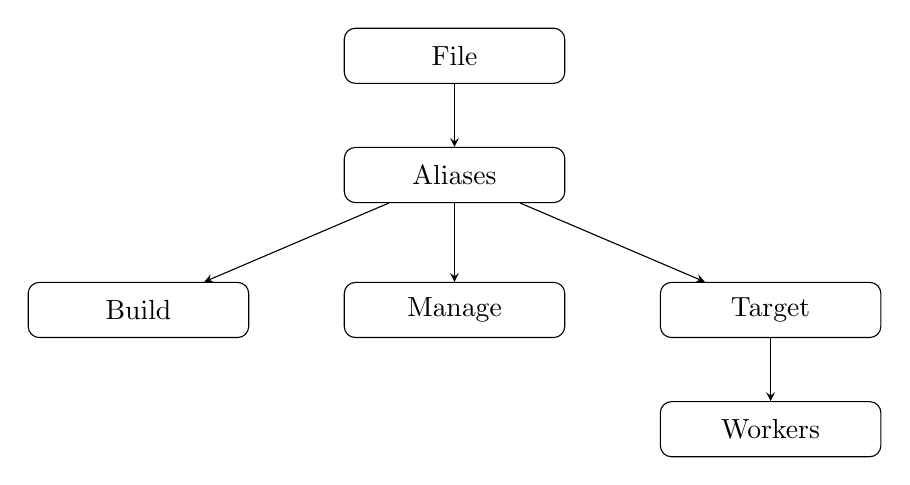
\begin{tikzpicture}[
            node distance=8mm,
            box/.style={
                draw,
                rounded corners,
                minimum width=28mm,
                minimum height=7mm,
                align=center
            },
            arrow/.style={->, >=stealth}
        ]
        \node[box] (file) {File};
        \node[box, below=of file] (alias) {Aliases};

        \node[box, below left=10mm and 12mm of alias] (build) {Build};
        \node[box, below=10mm of alias] (manage) {Manage};
        \node[box, below right=10mm and 12mm of alias] (target) {Target};

        \node[box, below=of target] (worker) {Workers};

        \draw[arrow] (file) -- (alias);
        \draw[arrow] (alias) -- (build);
        \draw[arrow] (alias) -- (manage);
        \draw[arrow] (alias) -- (target);
        \draw[arrow] (target) -- (worker);
        \end{tikzpicture}
    \end{center}

    The exact order of independent operations is implementation-dependent unless an ordering is explicitly required by their semantics.

    \subsection{File Processing}\label{subsec:file-processing}

    File process parses the Staployfile and constructs its internal representation.
    The configuration file MUST be syntactically valid before any operation is executed.
    Syntax errors prevent further processing of the file.
    During this stage, blocks, attributes, labels, and nested blocks are identified according to the Staployfile syntax.
    The resulting configuration is then used as the input to alias, build, manage, and target processing.
    File processing does not itself execute build commands, shell hooks, or worker operations.

    \subsection{Alias Processing}\label{subsec:alias-processing}

    Alias process resolves aliases declared in the Staployfile.
    Aliases provide alternative references to workers and applications and may therefore be used by subsequent expressions.
    Worker aliases are resolved when evaluating worker expressions.
    Application aliases are resolved when evaluating application references.
    An alias MUST resolve to a valid object of the corresponding type before it can be used.
    Alias resolution may involve additional expressions, including \texttt{where} conditions and \texttt{shell:} expressions where permitted.
    The result of alias processing is not itself an operation.
    It provides resolved references for subsequent processing stages.

    \subsection{Build Processing}\label{subsec:build-processing}

    Build process produces application artifacts from \texttt{build} blocks.
    A build is first resolved into its application, version, environment, target architectures, and output paths.
    Build-level commands and target-specific commands are then executed as required by the build definition.
    The resulting files are collected from the selected architecture target and the corresponding \texttt{share} target.
    The files specified by the \texttt{executable} attribute identify executable files in the resulting artifact.
    The values of this attribute are file names, not source paths.
    A build may produce artifacts for multiple target architectures.
    For example:

    \begin{center}
        %! suppress = MissingLabel
        \begin{verbatim}
            build "my-app" {
               output_dir = "./build"

               executable = [
               "my-app"
               ]

               share {
                  path = "./resources"
               }

               x86_64 {
                  path = "./bin/amd64"
               }

               aarch64 {
                  path = "./bin/arm64"
               }
            }
        \end{verbatim}
    \end{center}

    The resulting artifacts are made available to subsequent operations such as \texttt{upload}, \texttt{push\_only}, and \texttt{deploy}.
    If a required build input, target, or artifact cannot be resolved, build processing fails and the affected operation is not executed.

    \subsection{Manage Processing}\label{subsec:manage-processing}

    Manage process executes operations defined by \texttt{manage} blocks.
    The application identified by the \texttt{manage} block is resolved before the corresponding operation is performed.
    The operations modify or retrieve application data associated with the local Staploy server:

    \begin{itemize}
        \item \texttt{create} creates an application.
        \item \texttt{upload} transfers a local application package to the local server.
        \item \texttt{delete} removes application versions from the local server.
        \item \texttt{pull} retrieves an application package from an external Staploy repository and registers it in the local server.
    \end{itemize}

    For operations that require an application package, the required application and version are resolved before execution.
    Manage processing does not directly perform worker operations.
    Its scope is the application repository maintained by the Staploy server.

    \subsection{Target Processing}\label{subsec:target-processing}

    Target process executes operations defined by \texttt{target} blocks against selected workers.
    Worker selection is performed before the target operations are executed.
    The initial worker set is obtained from the \texttt{workers} attribute.
    If a \texttt{where} block is present, its conditions are applied to the selected workers and only workers satisfying all conditions remain in the target set.
    For each selected worker, the application and version required by the operation are resolved before the operation is submitted to the worker.
    Target operations are then executed according to the operation specified in the target block:

    \begin{itemize}
        \item \texttt{deploy} pushes and activates an application version.
        \item \texttt{push\_only} pushes an application version without activating it.
        \item \texttt{set\_active} activates an already available application version.
        \item \texttt{unset} clears the active application version.
        \item \texttt{remove} removes application versions from the worker.
        \item \texttt{disconnect} disconnects the worker from the server.
    \end{itemize}

    Shell hooks associated with a target operation are executed as part of target processing.
    A failure affecting one worker does not inherently imply that operations for other selected workers are canceled.
    The handling of individual and partial failures is defined by the error semantics.


    \section{Resolution Semantics}\label{sec:resolution-semantics}

    Resolution is the process of converting references and expressions in a Staployfile into concrete objects used during execution.
    Resolution is performed separately for workers, applications, aliases, and build artifacts.
    The result of each resolution MUST satisfy the constraints applicable to the corresponding object.
    Resolution does not itself perform an operation on a worker or modify the local Staploy server.
    It produces the concrete values required by subsequent execution stages.

    \subsection{Worker Resolution}\label{subsec:worker-resolution}

    Worker resolution converts worker expressions into a set of concrete workers.
    A worker expression may identify a worker directly by its ID or name, or indirectly through a group or worker alias.

    For example:

    \begin{center}
        %! suppress = MissingLabel
        \begin{verbatim}
            target "production" {
               workers = [
               "worker-01",
               "worker-02",
               "group:production",
               "alias:production-workers"
               ]

               ...
            }
        \end{verbatim}
    \end{center}

    The following forms are supported:

    \begin{itemize}
        \item A worker ID resolves to the corresponding worker.
        \item A worker name resolves to the corresponding worker.
        \item A \texttt{group:} expression resolves to all workers belonging to the specified group.
        \item An \texttt{alias:} expression resolves according to the corresponding worker alias.
    \end{itemize}

    If multiple expressions resolve to the same worker, the worker MUST occur only once in the resulting worker set.
    If an expression cannot be resolved, the target resolution fails.
    After the initial worker expressions have been resolved, a \texttt{where} block, when present, is applied to the resulting worker set.

    \subsection{Application Resolution}\label{subsec:application-resolution}

    Application resolution converts an application reference into a concrete application and, when required, a concrete application version.
    An application may be referenced directly by its name or indirectly through an application alias.
    For operations that require a version, the version may be explicitly specified:

    \begin{center}
        %! suppress = MissingLabel
        \begin{verbatim}
            deploy "my-app" {
               version = "1.2.0"
            }
        \end{verbatim}
    \end{center}

    When the version is omitted, Staploy resolves an applicable version according to the context of the operation.
    For target operations, version resolution may depend on the selected worker.
    This is necessary when the application contains multiple architecture-specific versions or artifacts.
    An application reference MUST resolve to an application available to the operation being performed.
    A requested version MUST also be available for the selected worker when the operation requires an architecture-compatible artifact.

    \subsection{Alias Resolution}\label{subsec:alias-resolution2}

    Alias resolution converts an alias reference into the object or expression represented by the alias.
    Worker aliases and application aliases are resolved independently according to their respective definitions.
    An alias may contain expressions that require further resolution.
    Alias resolution therefore proceeds recursively until the referenced object can be determined.

    For example:

    \begin{center}
        %! suppress = MissingLabel
        \begin{verbatim}
            alias {
               worker "production" {
                  ...
               }

               app "release" {
                  ...
               }
            }

            target "deploy-production" {
               workers = ["alias:production"]

               deploy "alias:release" {
                  ...
               }
            }
        \end{verbatim}
    \end{center}

    An alias MUST resolve to an object of the expected type.
    A worker alias cannot be used where an application reference is required, and an application alias cannot be used as a worker expression.
    Alias resolution MUST terminate.
    Circular aliases or other references that prevent resolution from reaching a concrete object are invalid.
    Where an alias contains a \texttt{where} block, its conditions are evaluated against the corresponding application or worker objects according to the alias semantics.

    \subsection{Build Artifact Resolution}\label{subsec:build-artifact-resolution}

    Build artifact resolution determines the package or artifact to be used by an operation from the results of a \texttt{build} block.
    A build may produce artifacts for multiple target architectures.
    The applicable artifact is selected according to the architecture of the target worker when the operation is worker-specific.
    For example, a build may contain:

    \begin{center}
        %! suppress = MissingLabel
        \begin{verbatim}
            build "my-app" {
               output_dir = "./build"

               executable = [
               "my-app"
               ]

               share {
                  path = "./resources"
               }

               x86_64 {
                  path = "./bin/x86_64"
               }

               aarch64 {
                  path = "./bin/aarch64"
               }
            }
        \end{verbatim}
    \end{center}

    The \texttt{share} target contains files common to all architectures.
    Architecture-specific targets provide files applicable to their respective architectures.
    When resolving an artifact for a worker, Staploy selects the target corresponding to the worker's architecture and combines it with the common files from the \texttt{share} target.
    The names specified by the \texttt{executable} attribute identify executable files in the resulting artifact.
    They are file names and do not identify source paths.
    If no compatible build artifact exists for the selected worker, artifact resolution fails.

    \subsection{Resolution Constraints}\label{subsec:resolution-constraints}

    Resolution MUST produce an unambiguous and valid result before the corresponding operation is executed.
    The following constraints apply:

    \begin{itemize}
        \item A worker reference MUST resolve to an existing worker.
        \item A worker alias MUST resolve to a worker reference or worker set.
        \item An application reference MUST resolve to an existing application when the operation requires an existing application.
        \item An application alias MUST resolve to an application reference.
        \item A requested application version MUST exist when an existing version is required.
        \item A worker-specific application artifact MUST be compatible with the architecture of the selected worker.
        \item An alias MUST NOT form a circular resolution chain.
        \item A resolution MUST NOT silently produce an ambiguous result.
    \end{itemize}

    Resolution failures prevent the affected operation from being executed.
    For target operations involving multiple workers, resolution is performed in the context of each selected worker when the result depends on worker-specific properties such as architecture.
    Consequently, the same application reference may resolve to different concrete artifacts for different workers while still representing the same logical application and version.


    \section{Error Semantics}\label{sec:error-semantics}

    Staploy distinguishes errors according to the stage at which they occur.
    An error in one operation or worker does not necessarily terminate execution of the remaining operations.
    Unless otherwise specified, processing continues with the next applicable operation or worker after an error has been reported.

    \subsection{Syntax Errors}\label{subsec:syntax-errors}

    A syntax error occurs when a Staployfile cannot be parsed according to the Staployfile syntax.
    Examples include malformed blocks, invalid attribute syntax, invalid labels, and values that cannot be decoded into the expected configuration type.
    A syntax error prevents the affected Staployfile from being processed.
    No operation depending on a successfully parsed configuration is executed when parsing fails.

    \subsection{Resolution Errors}\label{subsec:resolution-errors}

    A resolution error occurs when a reference cannot be resolved to the object required by an operation.
    Examples include an unknown worker, unknown application, unavailable application version, or unresolved alias.
    For target processing, a failure to resolve worker expressions causes the affected target to be skipped.
    Similarly, failure to resolve an application or application version prevents the corresponding operation from being executed.
    Resolution errors are reported to the user and do not necessarily terminate processing of subsequent targets or operations.

    \subsection{Build Errors}\label{subsec:build-errors}

    A build error occurs when a requested build cannot produce a valid application artifact.
    Build errors may result from invalid build configuration, failure of a build command, missing build output, unsupported target architecture, or failure while packaging the resulting artifact.
    A failed build MUST NOT be used as a successfully produced artifact by a subsequent operation.
    The affected build operation is reported as failed.
    Other independent operations may continue unless execution of those operations depends on the failed artifact.

    \subsection{Execution Errors}\label{subsec:execution-errors}

    An execution error occurs while performing an operation after the required references have been resolved.
    Execution errors may occur during communication with a worker, application deployment, application activation, application removal, package transfer, or shell hook execution.
    For operations performed on multiple workers, an execution error affecting one worker does not terminate execution for the remaining workers.
    For example, if a deployment is requested for three workers and deployment fails on the first worker, the remaining workers are still processed.
    Shell hook failures have additional semantics.

    A failure of a \texttt{pre\_deploy} hook aborts the associated operation.
    The operation itself is not executed after the hook failure.
    A failure of a \texttt{post\_deploy} hook does not undo an operation that has already completed.
    The hook failure is reported separately.

    \subsection{Partial Failure}\label{subsec:partial-failure}

    A multi-worker operation may produce different results for different workers.
    Such a result is considered a partial failure when at least one worker succeeds and at least one worker fails.

    For example:

    \begin{center}
        %! suppress = MissingLabel
        \begin{verbatim}
            target "production" {
               workers = [
               "worker-01",
               "worker-02",
               "worker-03"
               ]

               deploy "my-app" {
                  version = "1.2.0"
               }
            }
        \end{verbatim}
    \end{center}

    If the operation succeeds on \texttt{worker-01} and \texttt{worker-02} but fails on \texttt{worker-03}, the operation has partially failed.
    A failed worker does not cause successful operations on other workers to be rolled back.
    Staploy does not provide transactional rollback across workers for target operations.
    Consequently, after a partial failure, different workers may be left in different states.
    The CLI reports failures for individual workers while continuing execution where possible.
    A partial failure therefore indicates that the requested operation was not uniformly completed across all selected workers; it does not imply that the operation failed for every worker.


    \section{Conformance}\label{sec:conformance}

    A Staploy implementation conforms to this specification if it accepts valid Staployfiles according to the syntax and semantics defined in this document and applies the corresponding resolution and execution semantics.
    An implementation MAY provide additional features, attributes, or expressions, provided that they do not change the meaning of constructs defined by this specification.

    \subsection{Valid Staployfiles}\label{subsec:valid-staployfiles}

    A Staployfile is valid when all of the following conditions are satisfied:

    \begin{itemize}
        \item The file conforms to the Staployfile syntax.
        \item All required attributes and labels are present.
        \item All attribute values can be decoded into their declared types.
        \item All references used by an operation can be resolved when the operation is executed.
        \item Alias references resolve to objects of the expected type.
        \item Worker expressions resolve to valid workers or worker sets.
        \item Application references resolve to valid applications where required.
        \item Application versions and build artifacts satisfy the constraints applicable to the operation.
        \item Build blocks contain sufficient information to produce the requested artifact.
    \end{itemize}

    A syntactically valid file may nevertheless fail during resolution, build, or execution.
    Validity of the Staployfile therefore does not imply that every operation contained in the file will succeed.
    For example, the following file may be syntactically valid even when the referenced worker is not currently available:

    \begin{center}
        %! suppress = MissingLabel
        \begin{verbatim}
            target "production" {
               workers = ["worker-01"]

               deploy "my-app" {
                  version = "1.2.0"
               }
            }
        \end{verbatim}
    \end{center}

    The failure to resolve or communicate with \texttt{worker-01} is an execution or resolution error rather than a syntax error.

    \subsection{Implementation Requirements}\label{subsec:implementation-requirements}

    A conforming implementation MUST:

    \begin{itemize}
        \item parse the Staployfile according to the syntax defined in this specification;
        \item distinguish worker references from application references according to their respective contexts;
        \item support worker and application alias resolution;
        \item evaluate \texttt{where} conditions according to the defined filter semantics;
        \item resolve build artifacts according to the target worker architecture where applicable;
        \item execute manage and target operations according to their defined semantics;
        \item execute shell hooks in the worker context;
        \item distinguish \texttt{pre\_deploy} and \texttt{post\_deploy} hook failures according to their respective semantics;
        \item report errors without incorrectly treating partial success as complete success;
        \item preserve successful operations when another worker subsequently fails, unless an operation explicitly defines rollback semantics.
    \end{itemize}

    A conforming implementation MUST NOT silently reinterpret a construct defined by this specification.
    In particular, an implementation MUST NOT treat an unresolved reference as a successfully resolved reference, execute an operation after a failed \texttt{pre\_deploy} hook, or report a partially successful multi-worker operation as uniformly successful.
    Implementations MAY differ in their user interface, logging format, concurrency model, transport implementation, and internal representation, provided that the observable behavior required by this specification remains equivalent.


    \section{Examples}\label{sec:examples}

    This section provides examples of common Staployfile configurations.
    The examples are intended to demonstrate how the constructs defined in this specification can be combined into practical workflows.

    \subsection{Minimal Staployfile}\label{subsec:minimal-staployfile}

    The following is a minimal Staployfile containing a single target operation:

    \begin{center}
        %! suppress = MissingLabel
        \begin{verbatim}
            target "production" {
               workers = ["worker-01"]

               set_active "my-app" {
                  version = "1.0.0"
               }
            }
        \end{verbatim}
    \end{center}

    This configuration selects \texttt{worker-01} and activates version \texttt{1.0.0} of \texttt{my-app}.

    \subsection{Multi-architecture Build}\label{subsec:multi-architecture-build}

    A build may contain architecture-specific targets together with files shared by all architectures.

    \begin{center}
        %! suppress = MissingLabel
        \begin{verbatim}
            build "my-app" {
               output_dir = "./build"

               executable = [
               "my-app",
               "helper"
               ]

               share {
                  path = "./resources"
               }

               x86_64 {
                  path = "./bin/x86_64"
               }

               aarch64 {
                  path = "./bin/aarch64"
               }

               riscv64 {
                  path = "./bin/riscv64"
               }
            }
        \end{verbatim}
    \end{center}

    The \texttt{share} target contains files common to every architecture.
    Each architecture-specific target supplies the files applicable to that architecture.
    The values of \texttt{executable} identify executable file names contained in the resulting artifact.

    \subsection{Worker Alias}\label{subsec:worker-alias2}

    A worker alias can be used to give a reusable name to a group of worker references.

    \begin{center}
        %! suppress = MissingLabel
        \begin{verbatim}
            alias {
               worker "production" {
                  workers = [
                  "worker-01",
                  "worker-02",
                  "worker-03"
                  ]
               }
            }

            target "deploy-production" {
               workers = ["alias:production"]

               deploy "my-app" {
                  version = "1.0.0"
               }
            }
        \end{verbatim}
    \end{center}

    The \texttt{alias:production} expression resolves to the workers defined by the \texttt{production} worker alias.
    Worker aliases are useful when the same set of workers is referenced by multiple targets.

    \subsection{App Alias}\label{subsec:app-alias2}

    Application aliases can be used to provide reusable application references and versions.

    \begin{center}
        %! suppress = MissingLabel
        \begin{verbatim}
            alias {
               app "release" {
                  name = "my-app"
                  version = "1.0.0"
               }
            }

            target "production" {
               workers = ["group:production"]

               deploy "alias:release" {}
            }
        \end{verbatim}
    \end{center}

    The \texttt{alias:release} expression resolves to the application and version specified by the alias.
    This allows the application version used by multiple operations to be changed in one place.

    \subsection{Build and Upload}\label{subsec:build-and-upload}

    A build artifact can be produced and subsequently uploaded to the local Staploy server.

    \begin{center}
        %! suppress = MissingLabel
        \begin{verbatim}
            build "my-app" {
               output_dir = "./build"
               version = "1.0.0"

               executable = [
               "my-app"
               ]

               x86_64 {
                  path = "./bin/x86_64"
               }

               aarch64 {
                  path = "./bin/aarch64"
               }
            }

            manage "my-app" {
               upload {
                  path = "./build/my-app_1.0.0.tar"
               }
            }
        \end{verbatim}
    \end{center}

    The \texttt{build} block produces the application artifact in the specified output directory.
    The \texttt{upload} operation then registers the locally produced package with the local Staploy server.
    The upload operation does not send the package to a worker.

    \subsection{Build, Upload, and Deploy}\label{subsec:build-upload-and-deploy}

    The following example combines building, uploading, and deployment into a single Staployfile.

    \begin{center}
        %! suppress = MissingLabel
        \begin{verbatim}
            build "my-app" {
               output_dir = "./build"
               version = "1.0.0"

               executable = [
               "my-app"
               ]

               share {
                  path = "./resources"
               }

               x86_64 {
                  path = "./bin/x86_64"
               }

               aarch64 {
                  path = "./bin/aarch64"
               }
            }

            manage "my-app" {
               upload {
                  path = "./build/my-app_1.0.0.tar"
               }
            }

            target "production" {
               workers = ["group:production"]

               deploy "my-app" {
                  version = "1.0.0"

                  pre_deploy  = "systemctl stop my-app"
                  post_deploy = "systemctl start my-app"
               }
            }
        \end{verbatim}
    \end{center}

    This configuration represents a complete local deployment workflow.
    First, the application is built for the requested architectures.
    The resulting package is then uploaded to the local Staploy server.
    Finally, the specified application version is deployed to all workers selected by \texttt{group:production}.
    During deployment, the \texttt{pre\_deploy} hook is executed before the deployment operation and the \texttt{post\_deploy} hook is executed after it.
    The build and upload stages operate on the local environment and Staploy server, while the target stage performs operations on the selected workers.

    \subsection{Complete Deployment Example}\label{subsec:complete-deployment-example}

    The following example demonstrates a complete deployment workflow using worker aliases, application aliases, worker filtering,
    shell-based values, multi-architecture builds, package upload, and target operations.

    \begin{center}
        \scriptsize
        %! suppress = MissingLabel
        \begin{verbatim}
            alias {
               worker "zmx-deploy" {
                  workers = ["group:all"]

                  where {
                     arch = ["x86_64", "arm", "aarch64", "mipsel"]
                  }
               }

               app "zmx-build" {
                  name    = "zmx"
                  version = "shell:git describe --tags --abbrev=0"
               }
            }

            build "alias:zmx-build" {
               output_dir = "zig-out"
               executable = ["zmx"]

               envs        = ["ZIG_PATH=/home/$USER/.local/share/zig/0.16.0"]
               lib_version = "shell:echo zig $($(echo $ZIG_PATH)/zig version)"
               pre_build   = "git pull --no-edit"

               x86_64 {
                  pre_build = <<-EOF
                     $ZIG_PATH/zig build \
                        -Doptimize=ReleaseSmall \
                        -Dtarget=x86_64-linux-musl \
                        --prefix ./zig-out/amd64
                  EOF
                  path = "zig-out/amd64/bin"
               }

               arm {
                  pre_build = <<-EOF
                     $ZIG_PATH/zig build \
                        -Doptimize=ReleaseSmall \
                        -Dtarget=arm-linux-musleabihf \
                        --prefix ./zig-out/arm
                  EOF
                  path = "zig-out/arm/bin"
               }

               aarch64 {
                  pre_build = <<-EOF
                     $ZIG_PATH/zig build \
                        -Doptimize=ReleaseSmall \
                        -Dtarget=aarch64-linux-musl \
                        --prefix ./zig-out/aarch64
                  EOF
                  path = "zig-out/aarch64/bin"
               }

               mipsel {
                  pre_build = <<-EOF
                     $ZIG_PATH/zig build \
                        -Doptimize=ReleaseSmall \
                        -Dtarget=mipsel-linux-musleabihf \
                        --prefix ./zig-out/mipsel
                  EOF
                  path = "zig-out/mipsel/bin"
               }
            }

            configure {
               address = "192.168.50.194"
               port = 18090
               enforce_uuid = false
            }

            manage "alias:zmx-build" {
               upload {}
            }

            target "upload_zmx" {
               workers = ["alias:zmx-deploy"]

               unset "alias:zmx-build" {
                  pre_deploy = "zmx k"
               }

               deploy "alias:zmx-build" {
                  post_deploy = "zmx v"
               }
            }
        \end{verbatim}
    \end{center}

    The example defines two aliases.
    The \texttt{zmx-deploy} worker alias initially selects all workers through the \texttt{group:all} expression and then restricts the resulting worker set to the architectures supported by the build.

    The \texttt{zmx-build} application alias identifies the application as \texttt{zmx}.
    Its version is obtained dynamically using a \texttt{shell:} expression, which retrieves the latest Git tag.
    The \texttt{build} block uses the application alias and produces architecture-specific artifacts for \texttt{x86\_64}, \texttt{arm}, \texttt{aarch64}, and \texttt{mipsel}.
    Each target invokes Zig with an architecture-specific compilation target and places the resulting executable in its corresponding output directory.
    The \texttt{lib\_version} attribute demonstrates another use of the \texttt{shell:} expression.
    Its value is generated by executing a command in the build environment.
    The \texttt{manage} block uploads the resulting package to the configured local Staploy server.

    Finally, the \texttt{upload\_zmx} target performs the deployment.
    The \texttt{unset} operation first removes the currently active version from each selected worker.
    Its \texttt{pre\_deploy} hook invokes the application's command to terminate or otherwise disable the currently running instance.
    The subsequent \texttt{deploy} operation pushes the newly built version and activates it.
    Its \texttt{post\_deploy} hook invokes the application again after activation.
    This example demonstrates how aliases, resolution, build processing, package management, worker filtering, and target execution can be combined into a single deployment workflow.

\end{document}